
Since the results of No-Core Shell Model calculations can show a variety of different convergence behaviors for different observables depending on the nucleus or the chosen models of the nuclear force, it is of large interest to develop extrapolation methods which capture the complexity of the resulting sequences and predict accurate values for various input sequences.

In this section, we provide the theoretical foundation of artificial neural networks, which have already been used in various other physical
applications, for example in modeling $\beta$-decay half lifes \cite{nnbetadecay} or nuclear charge radii \cite{Akkoyun_2013}.

\subsection{Introduction to Artificial Neural Networks}

An artificial neural network is a pattern recognition algorithm in the field of machine learning. The term \textit{neural network} refers to the original idea to mimic the learning mechanism in biological organisms.

Inside the human brain, countless cells called neurons are connected to each other in a highly complex system. The strengths of these synaptic connections often change in response to external stimuli. This change is how the process of learning takes place in living organisms \cite{Aggarwal2018}.

This learning mechanism is translated to a machine learning algorithm by using basic data processing units that model the behavior of neurons. Because of that, the basic units of an artificial neural network are called neurons as well. These neurons are linked via directed connections. If we wanted to model the structure of the brain more precicely, there would be no restrictions on which neuron could link to which, since this is the case in the brain. The machine learning counterpart to this is called a \textit{recurrent network}. The mathematical model of recurrent networks can get arbitrarily complex, such that we only look at neural networks where the neurons are grouped in different layers and only connections from one layer to the next are permitted. This is called a \textit{feedforward network}. Throughout this thesis, we only look at feedforward networks.

In a feedforward network, we hope that the layers correspond to rising levels of abstraction, such that the neurons in earlier layers may capture every detail of the input data and neurons in later layers may capture subpatterns in the input data.

The process of using neural networks to make predictions about data sets consists of multiple phases.
In general, we want to \textit{train} a neural network by using data sets with known predictions and use them to adjust the model parameters of the network to maximize the precision of the predictions. For that, we need a large data set of NCSM calculations with known predictions. We therefore use sequences that have converged enough so that the limit can be used as a prediction target. This set is called the \textit{training set}.
After training a network, the nets will be \textit{validated} using samples from a \textit{validation set}, which also has known prediction targets. By comparing the predictions of the network with the targets, we can quantify the quality of the network. In \autoref{fig:fitting}, we can see examples of networks, that underfit or overfit the training data, as well as a network that fits the training data well.

\begin{figure}[H]
  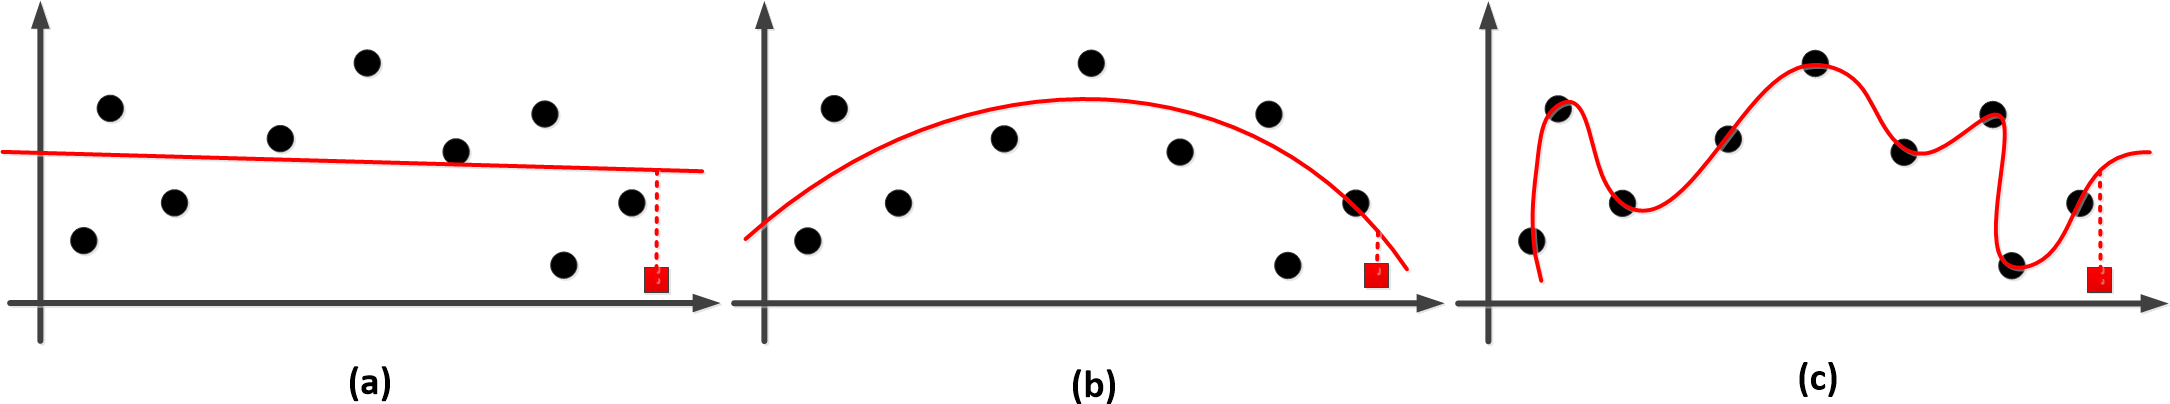
\includegraphics[width=\linewidth]{media/networkquality.png}
  \caption{Visualization of different qualities of network fits \cite{underfit}. The red line represents the data fit that was generated during training. The black dots symbolize the training samples and the red square denotes a validation sample. In the first example \textbf{(a)}, the network doesn't fit the training data well, such that the network prediction of the validation sample indicated by the meeting point of the dashed and solid red line is far away from the prediction target. Such a network would not qualify for evaluation. In the second example \textbf{(b)}, the network fits the data well, such that the prediction is close to the target. This network would meet the quality requirement. In the last example \textbf{(c)}, the network fits the training data too well, such that the prediction for the validation target is too unrealistic. This network would not meet the quality requirements.}
  \label{fig:fitting}
\end{figure}

After checking the quality of a network, we can then feed \textit{evaluation data} with unknown prediction targets into the network and gain a network prediction.

\subsection{Structure and Mathematical Framework}

\begin{wrapfigure}{r}{5cm}
  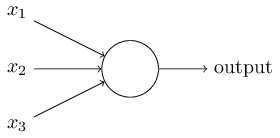
\includegraphics[width=5cm]{media/neuron.png}
  \caption{
    An example neuron with three input connections $x_1$, $x_2$ and
    $x_3$ and an output connection. \cite{nielsen}
  }
  \label{fig:neuron}
\end{wrapfigure}
To understand how an artificial neural network processes large amounts of data,
we must first discuss the structure of such networks.

In an ANN, the basic data processing unit is a neuron. Its only job is to take
input signals from directed connections to other neurons and process these inputs to generate an output signal, which can itself be connected to the input of other neurons. In \autoref{fig:neuron}, a sample neuron is depicted.

The activation $a$ of a neuron is computed by adding the input signals $x_j$ multiplied with connection weights $w_j$, representing the strength of the connection. This weighted sum is then added to a neuron bias $b$ and normalized using an activation function $\sigma$, yielding

\begin{equation}
  a = \sigma\left(\sum_j w_j x_j + b\right).
\end{equation}
In most use-cases, the activation function $\sigma$ is chosen such that the
neuron outputs are restricted to subsets of $\R$. To force neuron activations
to lie in $(0,1)$, one can use the sigmoid function
$\sigma(z) = [1+\exp(-z)]^{-1}$.

In feedforward neural networks, neurons are organized in layers 1 to $N$.
In each layer $n$, there are $L^{(n)}$ neurons and the neurons have an outbound connection to every neuron in layer $n+1$.
The $L^{(1)}$ neurons of layer 1 have no input connections and can be used to directly feed $L^{(1)}$-dimensional input data to the network.
The first layer of a neural network is thus called the \textit{input layer}.
When we feed $L^{(1)}$-dimensional data into the network, it propagates forward, layer-by-layer until the last layer, where the activations can be viewed as the processed output of the network. The last layer is thus called the \textit{output layer}.
The layers between the input and the output layer are called \textit{hidden layers}, since the activation of those neurons are neither direct inputs nor outputs of the data processing. In \autoref{fig:nn}, we can see a sample feed forward neural network.

\begin{figure}[H]
  \centering
  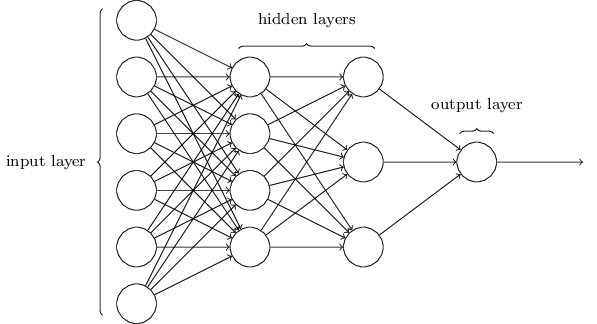
\includegraphics[width=0.7\textwidth]{media/network.png}
  \caption{A neural network with four layers \cite{nielsen}. Here, there are 6 neuron in the input layer ($L^{(1)} = 6$), 3 neurons in each hidden layer ($L^{(2)} = L^{(3)} = 3$) and one output neuron in the output layer ($L^{(4)}=1$). The connection between the neurons are limited to adjacent layers and information is only flowing from left to right. The depicted network is thus a feedforward network.}
  \label{fig:nn}
\end{figure}

Now, let $\vec{a}^{(n)} = (a_1, a_2, \dotsb, a_{L^{(n)}}) \in \R^{L^{(n)}}$ be the activations and $\vec{b}^{(n)} = (b_1, b_2, \dotsb, b_{L^{(n)}}) \in \R^{L^{(n)}}$ be the biases of the neurons in Layer $n$. For $1< n < N$, the activation of the neurons in layer $n+1$ can be functionally described by
\begin{align}
  A^{(n)}: \R^{L^{(n)}} & \longmapsto \R^{L^{(n+1)}}                                                        \\
  \vec{a}^{(n)}         & \longmapsto \vec{a}^{(n+1)} = \sigma\left(W^{(n)}\vec{a}^{(n)} +b^{(n+1)}\right).
\end{align}
Here, $W^{(n)} = (w^{(n)}_{ij})$ is the $(L^{(n+1)} \times L^{(n)})$-dimensional Matrix of the weights $w^{(n)}_{ij}$ from neuron $j$ in layer $n$ to neuron $i$ in layer $n+1$. Furthermore, the activation function $\sigma$ is applied elementwise. In that sense, one can view a neural network as a function
\begin{align}
  \label{eqn:ann_function}
  f: \R^{L^{(1)}} & \longmapsto \R^{L^{(N)}}                                                           \\
  x               & \longmapsto \left(A^{(N-1)} \circ \dotsb \circ A^{(2)}\right)(W^{(1)}x + b^{(2)}).
\end{align}
Before one constructs a feedforward artificial neural network, one has to think about the structure (i.e the count of layers and the count of neurons in each layer) and the used activation function. Those values have to be chosen such that the network can fulfill the data requirements and output the right data.

For example, if one uses an ANN to classify greyscale images of pixel-size $24\times 24$ into two classes $A$ and $B$ (this is called a \textit{binary classification problem}), one could choose $L^{(1)} = 24 \cdot 24 = 576$ and $L^{(N)} = 2$, such that each greyscale value can be fed into one input neuron and each output neuron corresponds to one of the two classes $A$ and $B$. If one restricts the output neurons to the range $(0, 1)$, one could extract the prediction of the network by choosing the neuron with the highest activation.
% Absatz über underfitting / overfitting

The function \eqref{eqn:ann_function} is dependent on the weights and biases of the connections and neurons. They can be viewed as internal parameters of $f$. When the network is initialized, they are often set to random values and the network will output random data. The challenge of machine learning is to apply algorithms on the outputs of the network to carefully adjust the weights and biases which results in the optimization of the network model \cite{nielsen}.

\subsection{Learning Process of a network}
\label{sec:sgd}
There are many ways to tackle the optimization process of neural networks. Training methods all rely on evaluating the outputs of some given inputs and comparing them to the values that \textit{should} be output by the network.

To quantify the performance of a given network $f$, we define a \textit{loss function} which depends on given inputs $x_1, x_2, \dots, x_n \in \R^{L^{(1)}}$, their desired outputs $o_1, o_2, \dots, o_n \in \R^{L^{(N)}}$ and, most importantly, the weights $w$ and the biases $b$ of the network, by
\begin{equation}
  \label{eqn:mseloss}
  C(w, b) = \frac{1}{n}\sum_{i=1}^{n}\norm{f(x_i)-o_i}^2.
\end{equation}
Note that the loss function is always positive and only zero, when the network predicts the correct output for every input. There are many ways to choose a loss function that has these properties. The function \eqref{eqn:mseloss} is called the \textit{mean squared error} (MSE) and is used throughout this thesis as the loss function.

Using this terminology, we can translate the optimization process of a network to a well-posed problem of finding the minimum of a function. Usually, the number of dimensions is too high to compute the minimum of the loss function analytically. One has to rely on numerical methods to find a local minimum of \eqref{eqn:mseloss}. A basic numerical algorithm that is used in machine learning is called \textit{gradient descent}. Even though this algorithm is very simplistic, it provides the basis for more sophisticated optimization algorithms such as the \textit{AdamW algorithm}, which is used in this thesis.

The gradient descend method is an iterative method that can be used to find a local minimum of an arbitrary differentiable function $f: \R^n \mapsto \R, x \mapsto f(x)$. Starting from a point $x^{(0)} \in \R^n$, we iteratively adjust the value by a finite amount $\Delta x$. The function will change by
\begin{equation}
  \label{eqn:approx}
  \Delta f \approx \frac{\partial f}{\partial x_1} \Delta x_1 + \dots + \frac{\partial f}{\partial x_2} \Delta x_2 = (\nabla f)(x) \cdot \Delta x.
\end{equation}

If we choose $\Delta x = -\eta (\nabla f)(x)$, with a small positive parameter $\eta$ called the \textit{learning rate}, we can force the right hand side of \eqref{eqn:approx} to be negative. In that way, if we adjust $x$ by $\Delta x$, we can ensure that the new function value at $x^{(1)} = x^{(0)}+ \Delta x$ will be smaller, if the approximation in \eqref{eqn:approx} is good enough. For that, it is important to carefully choose the value of $\eta$ small enough, but not too small. If the step size is too small, the new value will not have changed much and the total amount of steps must be increased to obtain a reasonable optimization.

Applied to the loss function \eqref{eqn:mseloss}, we get the iteration rule
\begin{align}
  w_i & \mapsto w_i' = w_i - \eta \frac{\partial C}{\partial w_i}, \\
  b_i & \mapsto b_i' = b_i - \eta \frac{\partial C}{\partial b_i}.
\end{align}

Since the cost function depends on every input $x_i$, it is computationally infeasible to calculate the gradient of the loss function directly. Therefore, we employ the \textit{stochastic gradient descent} algorithm. The idea is to approximate the gradient of the loss function by dividing the sample set into batches and calculating the gradient only using a single batch of samples. The resulting gradient will be used to adjust the weights and biases. This allows for more steps to be taken with a single iteration over the training data set, but the steps themselves are not as accurate as with gradient descent. An iteration over the whole training data set is commonly called an \textit{epoch}. The training of a single network can be done by specifying a total amount of training \textit{epochs}, or by specifying a \textit{threshold} for the loss function for when the training should end.

To compute the gradient of the loss function for a single training sample $x$, a classical backpropagation algorithm is used. The derivative of the loss function
\begin{equation}
  \label{eqn:singleloss}
  C_x(w, b) = \norm{a_i^{(N)}-o_i}^2
\end{equation}
with respect to a weight $w_{ij}^{(N-1)}$ from the $j$-th neuron in the second last layer to the $i$-th neuron in the last layer is calculated using the chain rule to
\begin{equation}
  \frac{\partial C_x}{\partial w_{ij}^{(N-1)}} = \frac{\partial C}{\partial a_i^{(N)}}\frac{\partial a_i^{(N)}}{\partial z_i^{(N)}} \frac{\partial z_i^{(N)}}{\partial w_{ij}^{(N-1)}},
\end{equation}
where $z_i^{(n)} = \sum_{j=1} w_{ij}^{(n-1)}a_j^{(n-1)}+b_i^{(n)}$ is the activation of neuron $i$ in layer $n$ before it is fed into the activation function. Using the Loss function from \eqref{eqn:singleloss}, we get
\begin{equation}
  \frac{\partial C_x}{\partial w_{ij}^{(N-1)}} = 2(a_i^{(N)}-o_i^{(N)}) \cdot \sigma'(z_i^{(N)}) \cdot a_j^{(N-1)}.
\end{equation}
Analogously, the derivative of $C_x$ with respect to the bias $b_i^{(N)}$ is given by
\begin{equation}
  \frac{\partial C_x}{\partial b_i^{(N)}} = 2(a_i^{(N)}-o_i^{(N)}) \cdot \sigma'(z_i^{(N)}).
\end{equation}
These equations can be used to adjust the weights of the second last layer, as well as the biases of the last. Since we also need the derivative with respect to weights and biases in the earlier layers, we can use the clever trick of applying this step iteratively to one layer backwards at a time. This is why this algorithm is called backpropagation. To compute those derivatives, we need to know how the loss function changes if activations in the second last layer change. This is given by
\begin{equation}
  \frac{\partial C_x}{\partial a_j^{(N-1)}} =\sum_{i=1}^{L^{N}} 2(a_i^{(N)}-o_i^{(N)}) \cdot \sigma'(z_i^{(N)}) \cdot w_{ij}^{(N-1)}.
\end{equation}
We can use this derivative to calculate derivatives of the loss function with respect to earlier layers and iteratively determine the gradient of $C_x$. The gradient of the whole loss function $C$ is then given by the average
\begin{equation}
  \nabla C = \sum_{x} \nabla C_x
\end{equation}
over all training samples in the batch \cite{nielsen}.
